% zed_base_arch.tex
% Hardware architecture of zed_base v7 (ZedBoard, Zynq-7020): block diagram, data flows,
% processing slot, address map and interrupts.
% Build: pdflatex zed_base_arch.tex
\documentclass[10pt]{article}
\usepackage[a4paper,landscape,margin=12mm]{geometry}
\usepackage{tikz}
\usetikzlibrary{arrows.meta,positioning,fit,backgrounds,calc,shapes.geometric}
\usepackage{booktabs}
\usepackage{caption}
\usepackage[T1]{fontenc}
\usepackage{lmodern}
\captionsetup{font=small}

% ---- colours: one per kind of connection ------------------------------------
\definecolor{cstream}{RGB}{31,119,180}   % AXI4-Stream video
\definecolor{cmm}{RGB}{214,39,40}        % AXI4 memory mapped (HP ports)
\definecolor{clite}{RGB}{110,110,110}    % AXI4-Lite control (GP0)
\definecolor{cvid}{RGB}{44,160,44}       % pixel bus / video out
\definecolor{ciic}{RGB}{255,127,14}      % I2C
\definecolor{cirq}{RGB}{148,103,189}     % interrupts
\definecolor{dpclk}{RGB}{255,247,220}    % camera PCLK domain
\definecolor{dvid}{RGB}{226,238,250}     % FCLK1 150 MHz domain
\definecolor{dpix}{RGB}{228,244,228}     % pixel clock domain
\definecolor{dacc}{RGB}{243,233,250}     % FCLK3 200 MHz domain
\definecolor{dps}{RGB}{238,238,238}      % processing system

\tikzset{
  blk/.style={draw,rounded corners=2pt,fill=white,align=center,font=\small,
              minimum height=9mm,minimum width=20mm,inner sep=2pt},
  ext/.style={blk,fill=black!8,draw=black!70},
  rtl/.style={blk,double,double distance=0.6pt},
  port/.style={draw,fill=white,font=\scriptsize,minimum height=5mm,minimum width=9mm,inner sep=1pt},
  st/.style={-{Latex[length=2.2mm]},cstream,line width=1.3pt},
  mm/.style={{Latex[length=2.2mm]}-{Latex[length=2.2mm]},cmm,line width=1.3pt},
  mmr/.style={-{Latex[length=2.2mm]},cmm,line width=1.3pt},
  lite/.style={-{Latex[length=1.6mm]},clite,dashed,line width=0.6pt},
  vid/.style={-{Latex[length=2mm]},cvid,line width=1.1pt},
  iic/.style={{Latex[length=1.6mm]}-{Latex[length=1.6mm]},ciic,densely dotted,line width=0.9pt},
  irq/.style={-{Latex[length=1.6mm]},cirq,line width=0.7pt},
  lbl/.style={font=\scriptsize,inner sep=1pt,fill=white,fill opacity=0.85,text opacity=1},
  dom/.style={rounded corners=4pt,inner sep=3mm},
  domlbl/.style={font=\scriptsize\itshape,anchor=north west,inner sep=2pt},
}

\begin{document}

% =============================================================================
\begin{figure}[p]
\centering
\resizebox{\textwidth}{!}{%
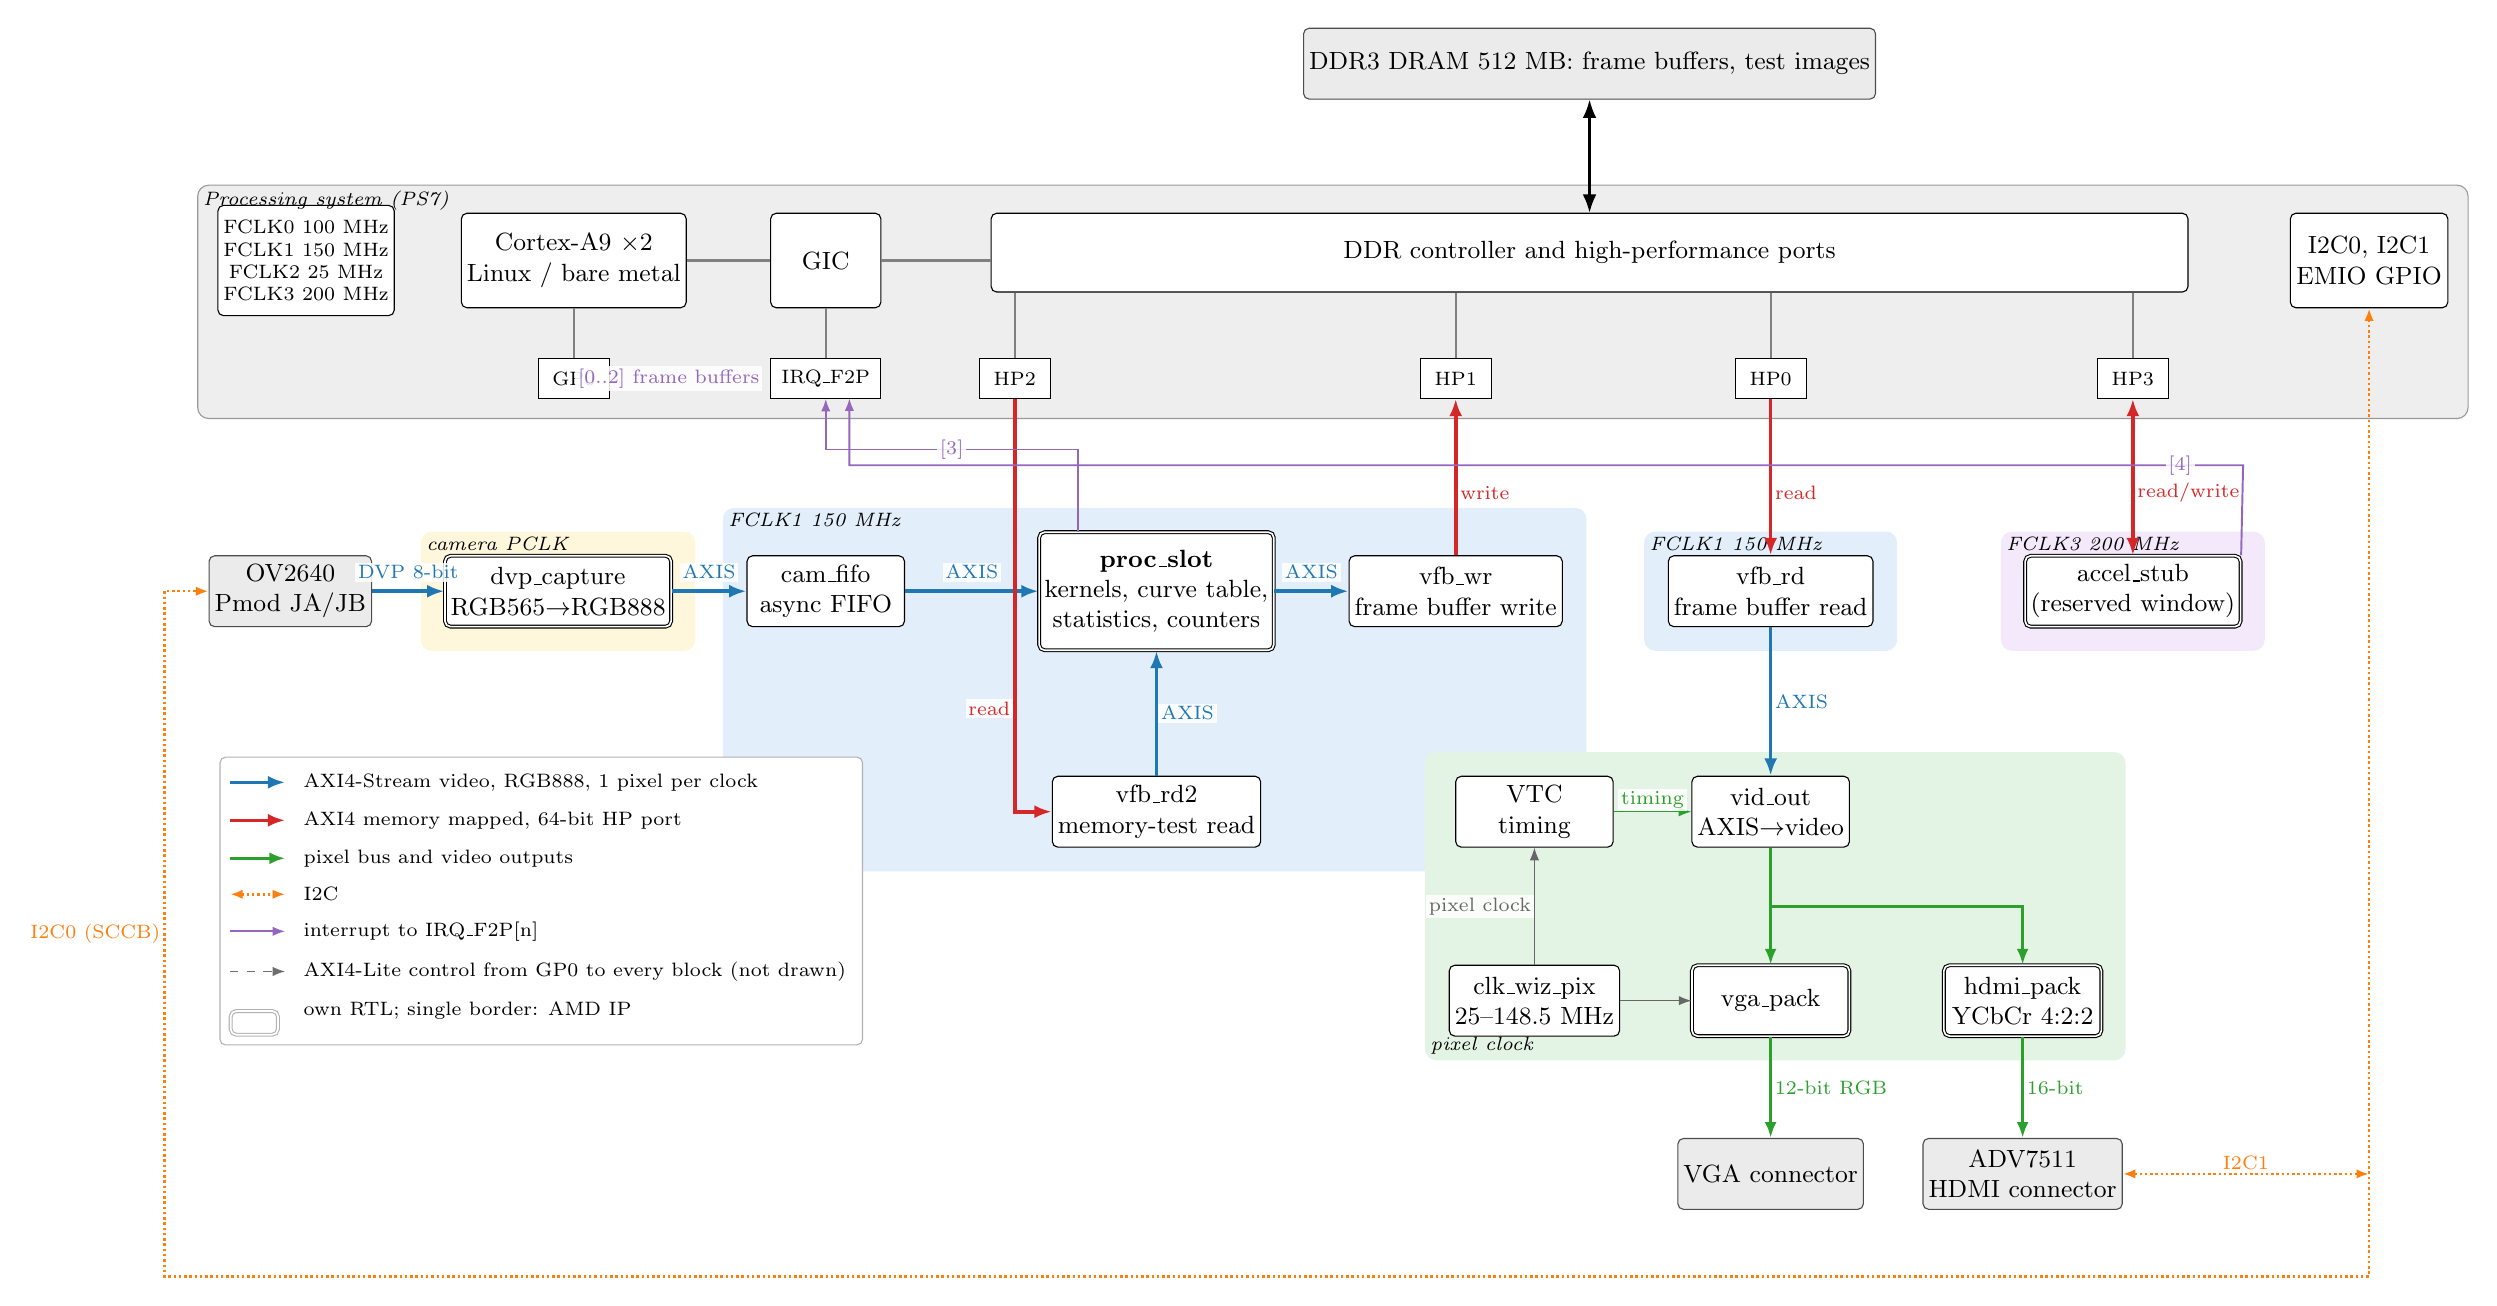
\begin{tikzpicture}
% ---- processing system (top band) -------------------------------------------------
\node[blk,minimum width=19mm,minimum height=14mm,font=\scriptsize] (clk) at (1.4,-1.0) {FCLK0 100 MHz\\FCLK1 150 MHz\\FCLK2 25 MHz\\FCLK3 200 MHz};
\node[blk,minimum width=26mm,minimum height=12mm] (cpu) at (4.8,-1.0) {Cortex-A9 $\times 2$\\Linux / bare metal};
\node[blk,minimum width=14mm,minimum height=12mm] (gic) at (8.0,-1.0) {GIC};
\node[blk,minimum width=152mm,minimum height=10mm] (ddrc) at (17.7,-0.9) {DDR controller and high-performance ports};
\node[blk,minimum width=20mm,minimum height=12mm] (periph) at (27.6,-1.0) {I2C0, I2C1\\EMIO GPIO};
\node[port] (gp0)  at (4.8,-2.5)  {GP0};
\node[port,minimum width=14mm] (f2p) at (8.0,-2.5) {IRQ\_F2P};
\node[port] (hp2)  at (10.4,-2.5) {HP2};
\node[port] (hp1)  at (16.0,-2.5) {HP1};
\node[port] (hp0)  at (20.0,-2.5) {HP0};
\node[port] (hp3)  at (24.6,-2.5) {HP3};
\draw[thick,gray] (cpu.south) -- (gp0.north);
\draw[thick,gray] (gic.south) -- (f2p.north);
\foreach \q in {hp0,hp1,hp2,hp3} \draw[thick,gray] (\q.north) -- (\q.north |- ddrc.south);
\draw[thick,gray] (cpu.east) -- (gic.west);
\draw[thick,gray] (gic.east) -- (gic.east -| ddrc.west);
\node[ext,minimum width=44mm] (dram) at (17.7,1.5) {DDR3 DRAM 512 MB: frame buffers, test images};
\draw[{Latex}-{Latex},thick] (dram) -- (ddrc);
\begin{scope}[on background layer]
  \node[fit=(clk)(cpu)(gic)(ddrc)(periph)(gp0)(hp3),fill=dps,draw=black!40,dom,inner sep=2.5mm] (ps) {};
\end{scope}
\node[domlbl] at (ps.north west) {Processing system (PS7)};

% ---- camera path ----------------------------------------------------------------------
\node[ext] (cam)   at (1.2,-5.2)  {OV2640\\Pmod JA/JB};
\node[rtl] (cap)   at (4.6,-5.2)  {dvp\_capture\\RGB565$\to$RGB888};
\node[blk] (fifo)  at (8.0,-5.2)  {cam\_fifo\\async FIFO};
\node[rtl,minimum width=28mm,minimum height=15mm] (slot) at (12.2,-5.2) {\textbf{proc\_slot}\\kernels, curve table,\\statistics, counters};
\node[blk] (vfbwr) at (16.0,-5.2) {vfb\_wr\\frame buffer write};
\node[blk] (vfbrd2) at (12.2,-8.0) {vfb\_rd2\\memory-test read};

% ---- display path ---------------------------------------------------------------------
\node[blk] (vfbrd)  at (20.0,-5.2)  {vfb\_rd\\frame buffer read};
\node[blk] (vidout) at (20.0,-8.0)  {vid\_out\\AXIS$\to$video};
\node[blk] (vtc)    at (17.0,-8.0)  {VTC\\timing};
\node[blk] (clkw)   at (17.0,-10.4) {clk\_wiz\_pix\\25--148.5 MHz};
\node[rtl] (vga)    at (20.0,-10.4) {vga\_pack};
\node[rtl] (hdmi)   at (23.2,-10.4) {hdmi\_pack\\YCbCr 4:2:2};
\node[ext] (vgaout) at (20.0,-12.6) {VGA connector};
\node[ext] (adv)    at (23.2,-12.6) {ADV7511\\HDMI connector};

% ---- accelerator window ----------------------------------------------------------------
\node[rtl] (acc) at (24.6,-5.2) {accel\_stub\\(reserved window)};

% ---- clock domains ----------------------------------------------------------------------
\begin{scope}[on background layer]
  \node[fit=(cap),fill=dpclk,dom] (dpc) {};
  \node[fit=(fifo)(slot)(vfbwr)(vfbrd2),fill=dvid,dom] (dv) {};
  \node[fit=(vfbrd),fill=dvid,dom] (dv2) {};
  \node[fit=(vtc)(clkw)(vga)(hdmi)(vidout),fill=dpix,dom] (dp) {};
  \node[fit=(acc),fill=dacc,dom] (da) {};
\end{scope}
\node[domlbl] at (dpc.north west) {camera PCLK};
\node[domlbl] at (dv.north west) {FCLK1 150 MHz};
\node[domlbl] at (dv2.north west) {FCLK1 150 MHz};
\node[domlbl,anchor=south west] at (dp.south west) {pixel clock};
\node[domlbl] at (da.north west) {FCLK3 200 MHz};

% ---- data paths ---------------------------------------------------------------------------
\draw[st] (cam) -- node[lbl,above=1mm]{DVP 8-bit} (cap);
\draw[st] (cap) -- node[lbl,above=1mm]{AXIS} (fifo);
\draw[st] (fifo) -- node[lbl,above=1mm]{AXIS} (slot);
\draw[st] (slot) -- node[lbl,above=1mm]{AXIS} (vfbwr);
\draw[st] (vfbrd2) -- node[lbl,right]{AXIS} (slot);
\draw[mmr] (vfbwr) -- node[lbl,right,pos=0.4]{write} (hp1);
\draw[mmr] (hp2.south) -- node[lbl,left,pos=0.75]{read} (10.4,-8.0) -- (vfbrd2.west);
\draw[mmr] (hp0) -- node[lbl,right,pos=0.6]{read} (vfbrd);
\draw[mm] (hp3) -- node[lbl,right,pos=0.6]{read/write} (acc);
\draw[st] (vfbrd) -- node[lbl,right]{AXIS} (vidout);
\draw[-{Latex[length=1.6mm]},cvid] (vtc) -- node[lbl,above]{timing} (vidout);
\draw[vid] (vidout.south) -- (20.0,-9.2) -- (vga.north);
\draw[vid] (20.0,-9.2) -| (hdmi.north);
\draw[vid] (vga) -- node[lbl,right]{12-bit RGB} (vgaout);
\draw[vid] (hdmi) -- node[lbl,right]{16-bit} (adv);
\draw[-{Latex[length=1.6mm]},black!60] (clkw) -- node[lbl,left]{pixel clock} (vtc);
\draw[-{Latex[length=1.6mm]},black!60] (clkw) -- (vga);

% ---- I2C (below everything) -----------------------------------------------------------------
\draw[iic] (periph.south) -- (27.6,-13.9) -- (-0.4,-13.9) -- node[lbl,left,pos=0.5]{I2C0 (SCCB)} (-0.4,-5.2) -- (cam.west);
\draw[iic] (27.6,-12.6) -- node[lbl,above]{I2C1} (adv.east);

% ---- interrupts ---------------------------------------------------------------------------------
\draw[irq] (11.2,-4.45) -- (11.2,-3.4) -- (8.0,-3.4) -- (f2p.south);
\node[lbl,text=cirq] at (9.6,-3.4) {[3]};
\draw[irq] (acc.north east) ++(0,0) -- (26.0,-3.6) -- (8.3,-3.6) -- (8.3,-2.75);
\node[lbl,text=cirq] at (25.2,-3.6) {[4]};
\node[lbl,text=cirq,anchor=east] at (7.2,-2.5) {[0..2] frame buffers};

% ---- legend -------------------------------------------------------------------------------------------
\matrix[draw=black!30,fill=white,rounded corners=2pt,inner sep=3pt,row sep=1.5pt,column sep=3pt,
        font=\scriptsize,anchor=north west,ampersand replacement=\&] at (0.3,-7.3) {
  \draw[st] (0,0) -- (7mm,0); \& \node[anchor=west]{AXI4-Stream video, RGB888, 1 pixel per clock}; \\
  \draw[mmr] (0,0) -- (7mm,0); \& \node[anchor=west]{AXI4 memory mapped, 64-bit HP port}; \\
  \draw[vid] (0,0) -- (7mm,0); \& \node[anchor=west]{pixel bus and video outputs}; \\
  \draw[iic] (0,0) -- (7mm,0); \& \node[anchor=west]{I2C}; \\
  \draw[irq] (0,0) -- (7mm,0); \& \node[anchor=west]{interrupt to IRQ\_F2P[n]}; \\
  \draw[lite] (0,0) -- (7mm,0); \& \node[anchor=west]{AXI4-Lite control from GP0 to every block (not drawn)}; \\
  \node[draw,double,double distance=0.6pt,minimum width=6mm,minimum height=3mm]{}; \& \node[anchor=west]{own RTL; single border: AMD IP}; \\
};
\end{tikzpicture}}
\caption{zed\_base v7 hardware architecture on the Zynq-7020.}
\label{fig:arch}
\end{figure}

% =============================================================================
\begin{figure}[p]
\centering
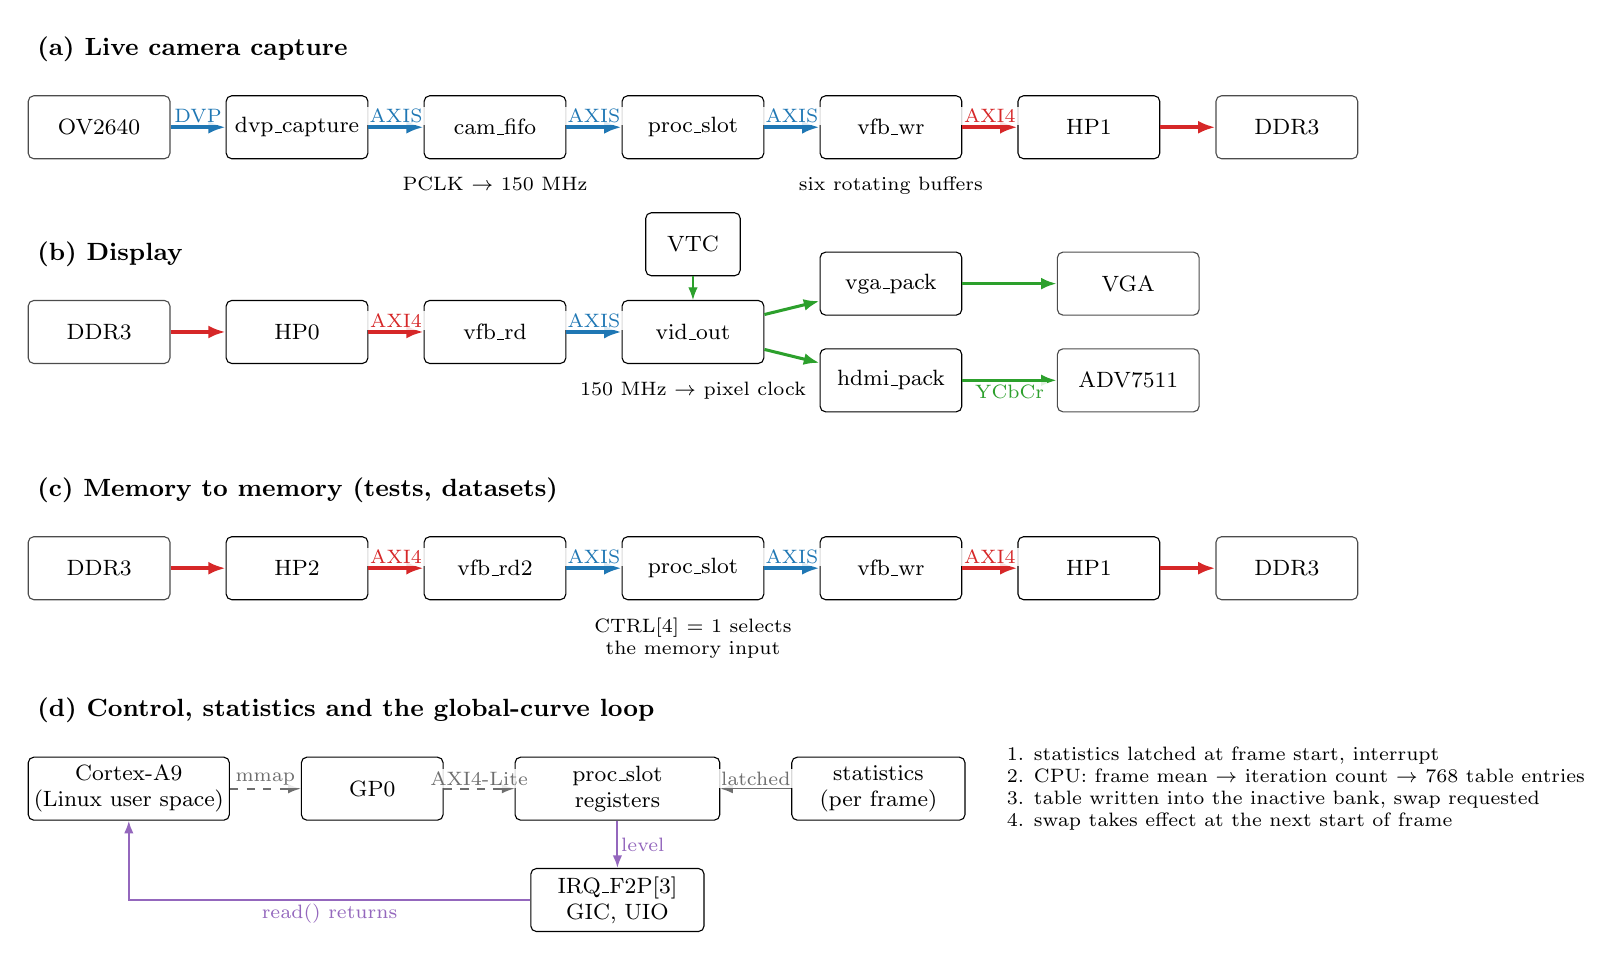
\begin{tikzpicture}[node distance=5mm and 7mm]
\tikzset{s/.style={blk,minimum width=18mm,minimum height=8mm,font=\footnotesize}}

% (a) live camera capture
\node[font=\small\bfseries,anchor=west] (ta) at (0,0) {(a) Live camera capture};
\node[ext,s,below=3mm of ta.south west,anchor=north west] (a1) {OV2640};
\node[s,right=of a1] (a2) {dvp\_capture};
\node[s,right=of a2] (a3) {cam\_fifo};
\node[s,right=of a3] (a4) {proc\_slot};
\node[s,right=of a4] (a5) {vfb\_wr};
\node[s,right=of a5] (a6) {HP1};
\node[ext,s,right=of a6] (a7) {DDR3};
\draw[st] (a1) -- node[lbl,above]{DVP} (a2);
\draw[st] (a2) -- node[lbl,above]{AXIS} (a3);
\draw[st] (a3) -- node[lbl,above]{AXIS} (a4);
\draw[st] (a4) -- node[lbl,above]{AXIS} (a5);
\draw[mmr] (a5) -- node[lbl,above]{AXI4} (a6);
\draw[mmr] (a6) -- (a7);
\node[font=\scriptsize,below=1mm of a3,align=center] {PCLK $\to$ 150 MHz};
\node[font=\scriptsize,below=1mm of a5,align=center] {six rotating buffers};

% (b) display
\node[font=\small\bfseries,anchor=west] (tb) at (0,-2.6) {(b) Display};
\node[ext,s,below=3mm of tb.south west,anchor=north west] (b1) {DDR3};
\node[s,right=of b1] (b2) {HP0};
\node[s,right=of b2] (b3) {vfb\_rd};
\node[s,right=of b3] (b4) {vid\_out};
\node[s,above right=-2mm and 7mm of b4] (b5) {vga\_pack};
\node[s,below right=-2mm and 7mm of b4] (b6) {hdmi\_pack};
\node[ext,s,right=12mm of b5] (b7) {VGA};
\node[ext,s,right=12mm of b6] (b8) {ADV7511};
\node[s,above=3mm of b4,minimum width=12mm] (b9) {VTC};
\draw[mmr] (b1) -- (b2);
\draw[mmr] (b2) -- node[lbl,above]{AXI4} (b3);
\draw[st] (b3) -- node[lbl,above]{AXIS} (b4);
\draw[vid] (b4) -- (b5);
\draw[vid] (b4) -- (b6);
\draw[vid] (b5) -- (b7);
\draw[vid] (b6) -- node[lbl,below]{YCbCr} (b8);
\draw[-{Latex[length=1.6mm]},cvid] (b9) -- (b4);
\node[font=\scriptsize,below=1mm of b4,align=center] {150 MHz $\to$ pixel clock};

% (c) memory test / datasets
\node[font=\small\bfseries,anchor=west] (tc) at (0,-5.6) {(c) Memory to memory (tests, datasets)};
\node[ext,s,below=3mm of tc.south west,anchor=north west] (c1) {DDR3};
\node[s,right=of c1] (c2) {HP2};
\node[s,right=of c2] (c3) {vfb\_rd2};
\node[s,right=of c3] (c4) {proc\_slot};
\node[s,right=of c4] (c5) {vfb\_wr};
\node[s,right=of c5] (c6) {HP1};
\node[ext,s,right=of c6] (c7) {DDR3};
\draw[mmr] (c1) -- (c2);
\draw[mmr] (c2) -- node[lbl,above]{AXI4} (c3);
\draw[st] (c3) -- node[lbl,above]{AXIS} (c4);
\draw[st] (c4) -- node[lbl,above]{AXIS} (c5);
\draw[mmr] (c5) -- node[lbl,above]{AXI4} (c6);
\draw[mmr] (c6) -- (c7);
\node[font=\scriptsize,below=1mm of c4,align=center] {CTRL[4] = 1 selects\\the memory input};

% (d) control and enhancement loop
\node[font=\small\bfseries,anchor=west] (td) at (0,-8.4) {(d) Control, statistics and the global-curve loop};
\node[s,below=3mm of td.south west,anchor=north west,minimum width=24mm] (d1) {Cortex-A9\\(Linux user space)};
\node[s,right=9mm of d1] (d2) {GP0};
\node[s,right=9mm of d2,minimum width=26mm] (d3) {proc\_slot\\registers};
\node[s,right=9mm of d3,minimum width=22mm] (d4) {statistics\\(per frame)};
\node[s,below=6mm of d3,minimum width=22mm] (d5) {IRQ\_F2P[3]\\GIC, UIO};
\draw[lite] (d1) -- node[lbl,above]{mmap} (d2);
\draw[lite] (d2) -- node[lbl,above]{AXI4-Lite} (d3);
\draw[-{Latex[length=1.6mm]},clite] (d4) -- node[lbl,above]{latched} (d3);
\draw[irq] (d3) -- node[lbl,right]{level} (d5);
\draw[irq] (d5) -| node[lbl,pos=0.25,below]{read() returns} (d1);
\node[font=\scriptsize,align=left,anchor=west] at ($(d4.east)+(4mm,0)$)
  {1. statistics latched at frame start, interrupt\\
   2. CPU: frame mean $\to$ iteration count $\to$ 768 table entries\\
   3. table written into the inactive bank, swap requested\\
   4. swap takes effect at the next start of frame};
\end{tikzpicture}
\caption{Data flows through the hardware.}
\label{fig:flows}
\end{figure}

% =============================================================================
\begin{figure}[p]
\centering
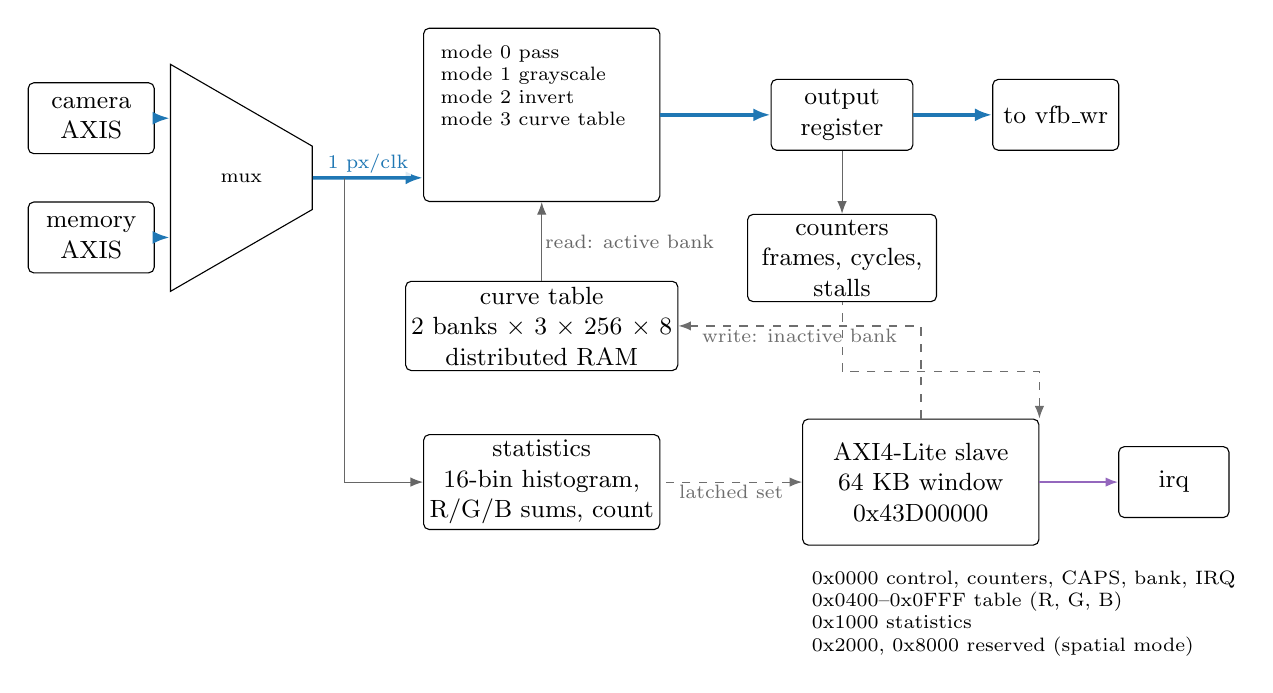
\begin{tikzpicture}[node distance=6mm and 9mm]
\node[blk,minimum width=16mm] (cami) {camera\\AXIS};
\node[blk,below=6mm of cami,minimum width=16mm] (memi) {memory\\AXIS};
\node[trapezium,draw,shape border rotate=270,minimum height=18mm,minimum width=6mm,font=\scriptsize,
      right=10mm of $(cami)!0.5!(memi)$] (mux) {mux};
\node[blk,right=14mm of mux,minimum width=30mm,minimum height=22mm,yshift=8mm] (ker) {};
\node[font=\scriptsize,align=left,anchor=north west] at ($(ker.north west)+(1mm,-1mm)$)
  {mode 0 pass\\mode 1 grayscale\\mode 2 invert\\mode 3 curve table};
\node[blk,right=14mm of ker,minimum width=18mm] (oreg) {output\\register};
\node[blk,right=10mm of oreg,minimum width=16mm] (out) {to vfb\_wr};
\node[blk,below=10mm of ker,minimum width=30mm] (lut) {curve table\\2 banks $\times$ 3 $\times$ 256 $\times$ 8\\distributed RAM};
\node[blk,below=8mm of lut,minimum width=30mm] (stat) {statistics\\16-bin histogram,\\R/G/B sums, count};
\node[blk,below=8mm of oreg,minimum width=24mm] (cnt) {counters\\frames, cycles,\\stalls};
\node[blk,right=18mm of stat,minimum width=30mm,minimum height=16mm] (regs) {AXI4-Lite slave\\64 KB window\\0x43D00000};
\node[blk,right=10mm of regs,minimum width=14mm] (irqo) {irq};

\draw[st] (cami) -- (cami -| mux.north west);
\draw[st] (memi) -- (memi -| mux.north west);
\draw[st] (mux) -- node[lbl,above]{1 px/clk} (ker.west |- mux);
\draw[st] (ker) -- (oreg);
\draw[st] (oreg) -- (out);
\draw[-{Latex[length=1.6mm]},black!60] (lut) -- node[lbl,right]{read: active bank} (ker);
\draw[-{Latex[length=1.6mm]},black!60] ($(mux.east)+(4mm,0)$) |- (stat.west);
\draw[-{Latex[length=1.6mm]},black!60] (oreg) -- (cnt);
\draw[lite] (regs.north) |- node[lbl,pos=0.75,below]{write: inactive bank} (lut.east);
\draw[{Latex[length=1.6mm]}-,clite,dashed] (regs.west) -- node[lbl,below]{latched set} (stat.east);
\draw[{Latex[length=1.6mm]}-,clite,dashed] (regs.north east) -- ++(0,6mm) -| (cnt.south);
\draw[irq] (regs) -- (irqo);
\node[font=\scriptsize,align=left,anchor=north west] at ($(regs.south west)+(0,-2mm)$)
  {0x0000 control, counters, CAPS, bank, IRQ\\0x0400--0x0FFF table (R, G, B)\\0x1000 statistics\\0x2000, 0x8000 reserved (spatial mode)};
\end{tikzpicture}
\caption{Inside proc\_slot v5 (FCLK1 150 MHz).}
\label{fig:slot}
\end{figure}

% =============================================================================
\begin{table}[p]
\centering
\caption{Address map, interrupts and clocks of shell v7.}
\label{tab:map}
\small
\begin{tabular}{@{}llll@{}}
\toprule
Address & Block & Interrupt & Clock \\
\midrule
0x41200000 & AXI GPIO, LEDs and switches & -- & FCLK0 100 MHz \\
0x41210000 & AXI GPIO, buttons & -- & FCLK0 100 MHz \\
0x43C00000 & vfb\_rd, display read (HP0) & IRQ\_F2P[0] & FCLK1 150 MHz \\
0x43C10000 & VTC, display timing & -- & pixel clock \\
0x43C20000 & vfb\_wr, camera and test write (HP1) & IRQ\_F2P[1] & FCLK1 150 MHz \\
0x43C30000 & clk\_wiz\_pix, pixel clock 25--148.5 MHz & -- & FCLK0 100 MHz (reference) \\
0x43C40000 & vfb\_rd2, memory-test read (HP2) & IRQ\_F2P[2] & FCLK1 150 MHz \\
0x43D00000 & proc\_slot, 64 KB & IRQ\_F2P[3] & FCLK1 150 MHz \\
0x43E00000 & accel window, 64 KB (stub, HP3 master) & IRQ\_F2P[4] & FCLK3 200 MHz \\
-- & dvp\_capture, cam\_fifo write side & -- & camera PCLK \\
-- & OV2640 SCCB / ADV7511 & PS I2C0 / I2C1 (EMIO) & -- \\
-- & frame buffer resets & EMIO GPIO 54--56 (57--61 spare) & -- \\
\bottomrule
\end{tabular}
\end{table}

\end{document}
